\section{Results}\label{sec:results}

We report the controls first, then the primary tail-small partition and its oracle bound, and finally the attribution, robustness and source checks that bound the finding.

\subsection{Literal truncation is negligible under standard overlap}\label{sec:res-trunc}

The premise that a tile boundary strips a small object of its pixels is false in this setting. Under the frozen 320-pixel tiling at overlap 0.25, not one of the 1{,}838 small audit objects, and none of the 38 tail-small objects, lacks a full view in some tile, even though a quarter of them (26.3\%) are crossed by at least one tile border (Table~\ref{tab:truncation}). A seam cut is not a lost object: in every audited case, whatever one tile bisects, a neighbouring tile holds whole.

\begin{table}[!htbp]
\scriptsize
\setlength{\tabcolsep}{4pt}
\caption{Literal truncation: objects with no full view in any SAHI tile (counts truncated/total). RicePest-30 rows count small objects ($<32^2$ in the 640-long-edge frame).}
\label{tab:truncation}
\begin{tabular*}{\textwidth}{@{\extracolsep{\fill}}llrrrrr}
\toprule
Data & $T$/stride & \shortstack{Train\\small} & \shortstack{Val\\small} & \shortstack{Audit\\small} & \shortstack{Audit\\tail-small} & \shortstack{Seam-cut\\(\%)} \\
\midrule
RicePest-30 & 320/240$^{\ast}$ & 0/21048 & 0/2680 & 0/1838 & 0/38 & 26.3 \\
RicePest-30 & 320/288 & 67/21048 & 10/2680 & 6/1838 & 0/38 & 26.2 \\
RicePest-30 & 320/320 & 1614/21048 & 214/2680 & 138/1838 & 3/38 & 19.3 \\
RicePest-30 & 256/192 & 0/21048 & 0/2680 & 0/1838 & 0/38 & 41.0 \\
RicePest-30 & 480/360 & 0/21048 & 0/2680 & 0/1838 & 0/38 & 12.5 \\
YST (native) & 640/480$^{\ast}$ & \multicolumn{4}{c}{31/8114 all objects (WF 0, MR 23, NC 8)} & 45.9 \\
YST (native) & 640/576 & \multicolumn{4}{c}{444/8114 all objects (WF 6, MR 308, NC 130)} & 38.6 \\
YST (native) & 640/640 & \multicolumn{4}{c}{1639/8114 all objects (WF 817, MR 571, NC 251)} & 25.4 \\
YST (native) & 512/384 & \multicolumn{4}{c}{147/8114 all objects (WF 0, MR 102, NC 45)} & 55.9 \\
\bottomrule
\end{tabular*}
\footnotetext{Seam-cut: share of objects crossed by at least one tile border (they still have a full view in a neighbouring tile). $^{\ast}$Frozen configuration. Overlap 0 is a positive control: it removes the redundancy that guarantees a full view.}
\end{table}


That the measurement would see truncation if it existed is confirmed by the positive control. Removing the overlap turns 138 of the 1{,}838 small audit objects (7.5\%) and 3 of the 38 tail-small objects into genuine no-full-view cases (Fig.~\ref{fig:truncation}); two alternative tile sizes keep truncation at exactly zero on the audit set, and on native-resolution YST only 31 of 8{,}114 objects are truncated at the frozen geometry, almost all of them the two larger-bodied classes rather than the whitefly. Truncation is therefore a real but near-zero quantity under standard overlap, which rules out missing pixels as the cause of the tail-small loss documented below and sends the question downstream.

\begin{figure}[!htbp]
    \centering
    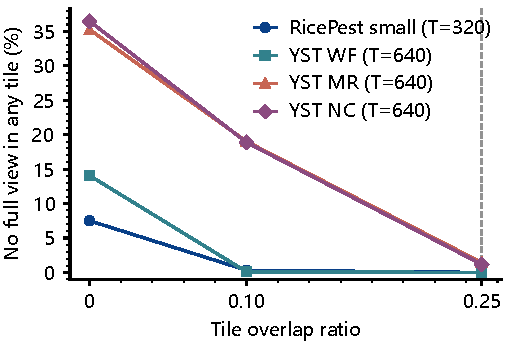
\includegraphics[width=0.65\textwidth,height=0.8\textheight,keepaspectratio]{../figures/fig_truncation_control.pdf}
    \caption{Literal truncation (no full view in any tile) against tile overlap: negative control at the frozen overlap 0.25 (dashed) and positive control at overlap 0. RicePest-30 small objects of the audit set ($T$=320 in the 640 frame) and YST objects per class (native $T$=640).}
    \label{fig:truncation}
\end{figure}

\subsection{Where tail-small objects are lost: the recovery-ceiling partition}\label{sec:res-partition}

With missing pixels excluded, the ledger locates the loss. For the pooled tail-small endpoint the dominant outcome among misses is that no candidate was ever formed: of the 27 tail-small misses, 16 (59\%, 95\% CI [41, 78]) have no same-class box at the 0.01 floor with IoU~$0.5$ in any view, against 2 lost only before the scored list and 9 recoverable after decoding (Table~\ref{tab:partition}). Head-small objects of the same nominal size class are the mirror image: 88\% of their 403 misses did produce a candidate, and they are lost at the merge (39\%) or below the score threshold (49\%), with only 12\% never forming a candidate. The tail-small endpoint is small and dominated by one leafhopper species, so this is a statement about the pooled audited set rather than a per-class law; we return to that limit in the discussion.

\begin{table}[!htbp]
\footnotesize
\caption{Recovery-ceiling partition of missed objects (YOLO11n).}
\label{tab:partition}
\begin{tabular}{lrrrrrr}
\toprule
Stratum, size & $N$ (groups) & Recall (\%) & Misses & No cand. & Pre-supp. & Post-hoc \\
\midrule
Tail $<32^2$ (primary) & 38 (27) & 28.9 & 27 & 16 (59) & 2 (7) & 9 (33) \\
\quad 95\% CI & & [12, 49] & & [41, 78] & [0, 18] & [17, 55] \\
\quad Tail $<16^2$ & 11 (5) & 9.1 & 10 & 7 & 2 & 1 \\
\quad Tail $16^2$--$32^2$ & 27 (24) & 37.0 & 17 & 9 (53) & 0 (0) & 8 (47) \\
Mid $<32^2$ & 114 (29) & 77.2 & 26 & 7 (27) & 5 (19) & 14 (54) \\
Head $<32^2$ & 1686 (257) & 76.1 & 403 & 47 (12) & 159 (39) & 197 (49) \\
\quad 95\% CI & & [74, 79] & & [8, 16] & [32, 46] & [42, 56] \\
Tail $\geq 32^2$ & 210 (156) & 58.1 & 88 & 40 (45) & 5 (6) & 43 (49) \\
Mid $\geq 32^2$ & 554 (251) & 71.1 & 160 & 67 (42) & 19 (12) & 74 (46) \\
Head $\geq 32^2$ & 1827 (332) & 88.2 & 215 & 50 (23) & 65 (30) & 100 (47) \\
All objects & 4429 (508) & 79.3 & 919 & 227 (25) & 255 (28) & 437 (48) \\
\bottomrule
\end{tabular}
\footnotetext{Group-disjoint audit set, frozen YOLO11n + SAHI ($T$=320, overlap 0.25, GREEDYNMM/IOS 0.5 at the 0.01 floor), operating point score $\geq$0.25 and 100 boxes per image. Miss columns: count (\% of misses); CI rows: 95\% cluster-bootstrap CI over audit groups; rates and CIs are omitted when a cell has $<$10 events or $<$5 groups. Size-matched contrast (tail-small vs head-small standardized to the tail size mix): no-candidate share difference 33.3 pp [16.7, 50.0], Holm $p$=0.013; pre-suppression-only -11.9 pp [-18.0, -5.2], Holm $p$=0.026; post-hoc-recoverable 9.6 pp [-3.7, 25.1], Holm $p$=0.149.}
\end{table}


The partition is visible as a single reversal between the two strata (Fig.~\ref{fig:partition}): for tail-small the no-candidate block is the tallest, whereas for head-small of the same size the pre-suppression and post-hoc blocks dominate and the no-candidate block is thin. Reading the 16 tail-small no-candidate misses individually, 7 produced no box at all, 5 produced a box of the wrong class, and 4 carry same-class evidence that only the multi-label read-out of the same forward pass exposes; and all 9 post-hoc-recoverable tail-small misses are threshold losses, none a cap loss. The practical consequence is already decided at this point: a majority of tail-small misses sit in the one category that no post-processing can reach, so effort spent on merging, thresholding or calibration is spent on the minority.

\begin{figure}[!htbp]
    \centering
    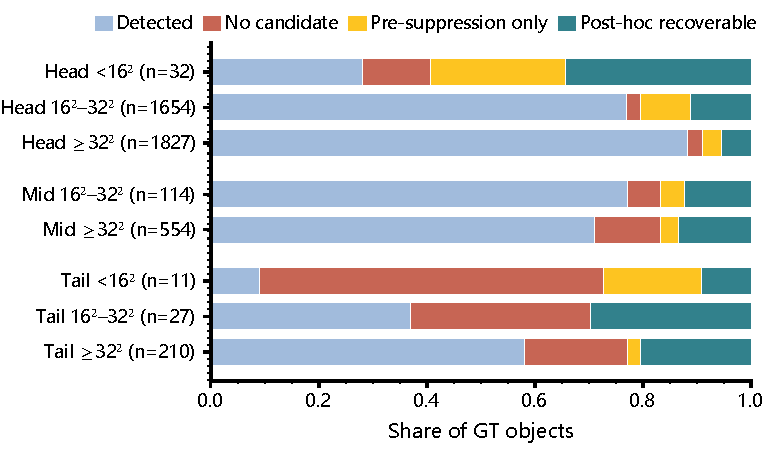
\includegraphics[width=0.98\textwidth,height=0.8\textheight,keepaspectratio]{../figures/fig_partition.pdf}
    \caption{Recovery-ceiling partition of every audit object (YOLO11n, SAHI $T$=320, overlap 0.25). Each bar splits the objects of one stratum and size bin into detected, no candidate, pre-suppression only and post-hoc recoverable.}
    \label{fig:partition}
\end{figure}

How much a better read-out could recover without a new detector is bounded by the oracle. For tail-small objects the oracle full-view read-out lifts recall from the emitted 28.9\% to only 31.6\%, a single additional object, so reordering the existing full-view evidence at fixed scores has almost no headroom (Fig.~\ref{fig:stage-survival}). Perfect rescoring of that evidence down to the floor would reach 57.9\%, and the remaining 42.1\% (16 objects) correspond exactly to the no-candidate mass that neither selection nor rescoring can touch. Head-small objects behave differently: a better read-out alone is worth up to 8.3 points (76.1\% to 84.4\%) and rescoring reaches 97.1\%, because their evidence is present and merely suppressed. The oracle thus certifies that the tail-small ceiling is set at candidate formation, not in the read-out.

\begin{figure}[!htbp]
    \centering
    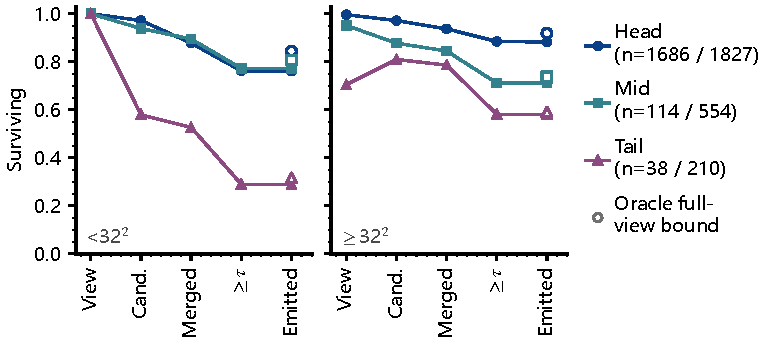
\includegraphics[width=0.98\textwidth,height=0.8\textheight,keepaspectratio]{../figures/fig_stage_survival.pdf}
    \caption{Stage-survival profile of the per-object ledger on the audit set (YOLO11n). Left: objects smaller than $32^2$; right: larger objects. Hollow markers: oracle full-view read-out (baseline detections plus every same-class candidate scoring at least 0.25 in a view that holds the whole object).}
    \label{fig:stage-survival}
\end{figure}

\subsection{The tail/head difference survives size matching}\label{sec:res-contrast}

A sceptic could argue that tail-small objects are simply smaller within the $<32^2$ band and that candidate formation fails on the smallest objects of any class. Matching the size distribution removes that explanation. Re-weighting head-small objects to the tail size mix, the no-candidate share is 38.2\% for tail against 4.9\% for size-matched head, a difference of $+33.3$ percentage points (95\% CI [16.7, 50.0], Holm $p=0.013$), while the pre-suppression-only share runs the other way at $-11.9$ points ([$-18.0$, $-5.2$], Holm $p=0.026$) and the post-hoc difference is not significant ($+9.6$ points, $p=0.149$); truncation stays at exactly zero in both strata (Fig.~\ref{fig:contrast}). At matched size, then, tail-small objects are lost before a candidate exists and head-small objects after, so the profile is not accounted for by size matching in this audit. We state this as the measured dissociation it is, not as a claim that every size-related mechanism has been ruled out.

\begin{figure}[!htbp]
    \centering
    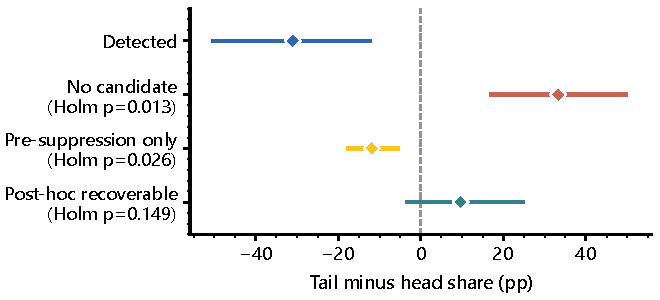
\includegraphics[width=0.85\textwidth,height=0.8\textheight,keepaspectratio]{../figures/fig_contrast.pdf}
    \caption{Size-matched frequency contrast: share of each outcome among tail-small objects minus the share among head-small objects re-weighted to the tail size mix (percentage points; bars: 95\% cluster-bootstrap CI over audit groups; Holm-adjusted $p$ from exact class-label permutation).}
    \label{fig:contrast}
\end{figure}

\subsection{The dominant stage is stable across the read-out, tiling and operating point}\label{sec:res-robust}

The location of the tail-small loss does not depend on the frozen configuration. Sweeping the merge rule, the tile size, the score threshold and the output cap, the tail-small no-candidate count stays between 13 and 20 of 38 throughout, so the candidate-formation bottleneck is not an artefact of any one read-out or threshold (Appendix~\ref{sec:app-sensitivity}, Table~\ref{tab:sensitivity}, Fig.~\ref{fig:sensitivity}). What does change with the read-out is the head-small profile: SAHI's union merge applied to the floor-level list creates most of the 159 head-small pre-suppression losses, and switching to an NMS merge removes 142 of them, which is why head-small recall is sensitive to the merge while tail-small recall is not. Slicing still matters for tail-small detection at the operating point, with full-image inference finding only 5 of 38 tail-small objects against 11 of 38 under slicing; the output cap bites only on dense head-class images and never constrains the tail. The robustness sweep therefore reinforces the partition rather than qualifying it: the tail-small ceiling is fixed upstream of the read-out, score threshold and cap that a deployer would adjust.

\subsection{The dominant stage is detector-dependent}\label{sec:res-detector}

Whether candidate formation dominates depends on the detector, and the second detector makes this explicit. Under the frozen read-out FCOS collapses for every stratum: trained for only six epochs it writes the full 300 boxes per view at the floor (1.85~million candidates over the 890 images, against 113{,}489 for YOLO11n), and SAHI's union merge fuses them into oversized boxes, so the merge stage, not candidate formation, dominates its losses (Fig.~\ref{fig:detectors}, Appendix Table~\ref{tab:partition-fcos}). This is a property of a dense low-score detector meeting a union merge, not of the tail. Once that merge artefact is read past, the detector-side quantity is genuinely smaller for FCOS: 9 to 10 of 38 tail-small objects have no candidate under any FCOS read-out, against 16 of 38 for YOLO11n, and only 8 of YOLO11n's 16 no-candidate tail-small objects are also no-candidate for FCOS. The size-matched frequency contrast replicates in direction on FCOS ($+11.1$ to $+14.1$ points, exact-permutation Holm $p=0.006$) though its magnitude is smaller and the group-bootstrap interval includes zero, so the dissociation is reproduced but not independently powered on the undertrained second detector. Candidate formation therefore carries the tail-small loss for YOLO11n specifically, and the dominant stage is contingent on the detector rather than universal.

\begin{figure}[!htbp]
    \centering
    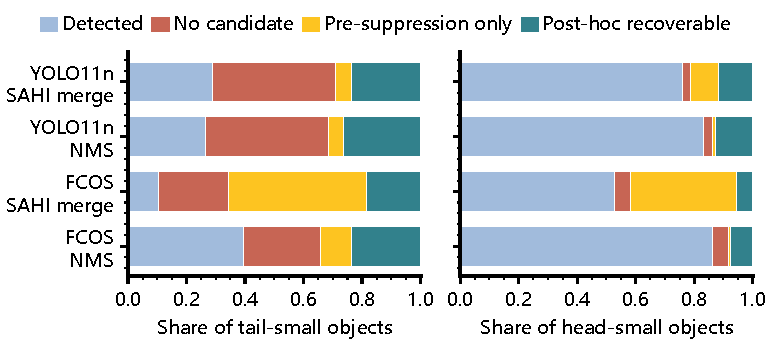
\includegraphics[width=0.98\textwidth,height=0.8\textheight,keepaspectratio]{../figures/fig_detectors.pdf}
    \caption{Cross-detector check: outcome shares of tail-small (left, 38 objects) and head-small (right, 1686 objects) audit objects for YOLO11n and FCOS-ResNet50-FPN under the frozen SAHI merge (GREEDYNMM-IOS at the 0.01 floor) and under an NMS-IoU 0.5 merge.}
    \label{fig:detectors}
\end{figure}

\subsection{Same-dump baselines recover exactly what the partition allows}\label{sec:res-methods}

If the partition is correct, a post-hoc method can only recover misses from the category its mechanism addresses, and this is what the baselines do when they re-read the identical candidate dump (Table~\ref{tab:methods}). Each method's parameters are fit by 5-fold group cross-fitting on the audit set, and every comparison is made at matched false positives, meaning one global score threshold per method chosen so that its total false positives do not exceed the frozen baseline's, so that recall gains cannot be bought with extra detections. Rescoring and calibration in the style of cross-view agreement~\citep{na2026crossview}, prior correction~\citep{pan2021norcal} and class$\times$size thresholds recover only post-hoc-recoverable misses: the per-class Na-style rescoring recovers 143 baseline misses at matched false positives, every one of them post-hoc-recoverable and none from the no-candidate or pre-suppression categories. Methods that instead replace the union merge with a per-location peak read-out recover pre-suppression-only misses, about 200 of them, and these are almost all head-small objects that the merge had absorbed. The gain from the peak read-out is real but it is a head-small gain: at matched false positives it lifts head-small recall from 76.1\% to 80.1\% and all-object recall from 79.3\% to 80.6\%, with the same effect whether it reads standard or multi-label evidence, so the improvement comes from discarding the union merge rather than from new evidence (Fig.~\ref{fig:methods}). None of the tested methods moves the tail-small no-candidate objects, as the oracle already required.

\begin{table}[!htbp]
\fontsize{6pt}{7pt}\selectfont
\caption{Same-dump post-processing methods on the audit set (YOLO11n; parameters fit by 5-fold group cross-fitting).}
\label{tab:methods}
\begin{tabular*}{\textwidth}{@{\extracolsep{\fill}}p{3cm}rrrrrrrrr}
\toprule
Method & \multicolumn{4}{c}{Own operating point} & \multicolumn{5}{c}{Matched false positives} \\ \cmidrule(lr){2-5}\cmidrule(lr){6-10} & R all & \shortstack{Tail\\small} & \shortstack{P\\head} & FP & R all & \shortstack{R head\\small} & \shortstack{Tail\\small} & \shortstack{Recov.\\P/H/N} & Lost \\
\midrule
SAHI baseline (frozen) & 79.3 & 11/38 & 54.6 & 3671 & 79.3 & 76.1 & 11/38 & 0/0/0 & 0 \\
NorCal-style prior correction & 79.1 & 11/38 & 55.1 & 3621 & 79.1 & 75.9 & 11/38 & 0/2/0 & 9 \\
Class$\times$size thresholds & 69.1 & 11/38 & 68.9 & 1715 & 78.5 & 75.7 & 14/38 & 0/31/0 & 64 \\
Na-style rescoring, class-agnostic & 77.5 & 10/38 & 61.3 & 2766 & 80.3 & 77.9 & 11/38 & 0/103/0 & 57 \\
Na-style rescoring, per class & 74.9 & 9/38 & 65.2 & 2151 & 80.2 & 78.4 & 11/38 & 0/143/0 & 102 \\
Multi-label evidence + SAHI merge + thr. & 69.2 & 12/38 & 68.9 & 1772 & 78.6 & 75.2 & 14/38 & 2/36/20 & 85 \\
Peak read-out on std evidence + thr. & 72.3 & 10/38 & 67.1 & 2016 & 80.6 & 80.1 & 14/38 & 201/13/0 & 153 \\
CCPR without class$\times$size thr. & 83.4 & 11/38 & 51.4 & 4497 & 81.0 & 81.1 & 8/38 & 207/3/1 & 132 \\
CCPR (multi-label peak read-out + thr.) & 72.6 & 11/38 & 67.1 & 2073 & 80.7 & 79.6 & 15/38 & 200/20/16 & 170 \\
\bottomrule
\end{tabular*}
\footnotetext{R: recall@0.5 (\%); P head: precision of emitted head-class boxes (\%); tail-small: detected/total. Matched FP: one global threshold per method chosen so that its total false positives do not exceed the baseline's. Recov.\ P/H/N: baseline misses recovered at matched FP, by the baseline's recovery-ceiling category (pre-suppression only / post-hoc recoverable / no candidate); Lost: baseline detections no longer detected.}
\end{table}


\begin{figure}[!htbp]
    \centering
    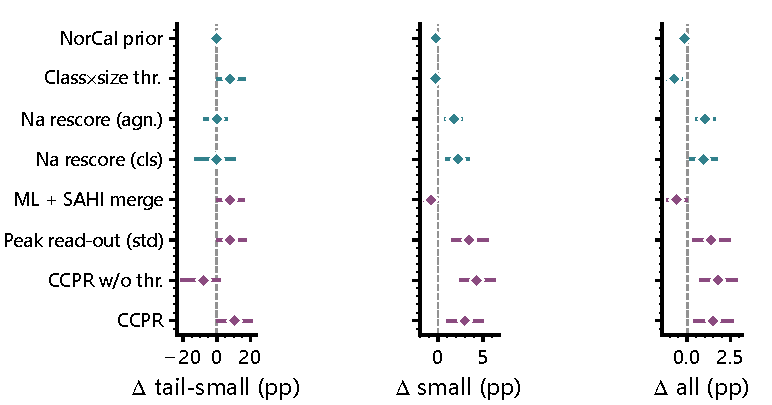
\includegraphics[width=0.98\textwidth,height=0.8\textheight,keepaspectratio]{../figures/fig_methods.pdf}
    \caption{Same-dump post-processing against the frozen SAHI baseline at matched false positives: paired difference in recall@0.5 (percentage points, 95\% cluster-bootstrap CI). Left to right: tail-small (38 objects), small (1838) and all (4429) audit objects. Teal: post-hoc rescoring/calibration; violet: read-out changes.}
    \label{fig:methods}
\end{figure}

The class-conditional peak read-out (CCPR) was pre-registered as a likely-null secondary increment, and the data confirm that expectation. Against class$\times$size calibration, CCPR adds no tail-small true positives at its own operating point (difference $0.0$ points, 95\% CI [$-11.1$, $9.1$]), and the matched-precision and matched-false-positive comparisons add $-1$ and $+1$ (Table~\ref{tab:ccpr}). Head non-inferiority passes at every operating point, but the first and third go criteria, at least five additional tail-small true positives and a recall interval excluding zero, both fail, so the planned decision is NO-GO: class$\times$size calibration already absorbs whatever tail-small gain CCPR could offer. An NMS-based comparator reaches the same NO-GO on both detectors, so the result is not an artefact of the frozen merge. The read-out increment is therefore reported as a negative result, which is the outcome the partition predicts once the tail-small loss is known to sit at candidate formation rather than in the read-out.

\begin{table}[!htbp]
\fontsize{5pt}{6pt}\selectfont
\caption{Pre-registered go/no-go test of CCPR against class$\times$size threshold calibration (audit set, YOLO11n).}
\label{tab:ccpr}
\begin{tabular*}{\textwidth}{@{\extracolsep{\fill}}lrrrrr}
\toprule
Comparison & \shortstack{Extra tail-\\small TP} & \shortstack{$\Delta$ tail-small\\recall, pp [95\% CI]} & \shortstack{$\Delta$ head recall, pp\\(one-sided 95\% LB)} & \shortstack{NI margin\\(pp)} & \shortstack{Criteria 1/2/3,\\Decision} \\
\midrule
Own operating points & +0 & +0.0 [-11.1, 9.1] & +3.7 (+2.7) & 1 & no/yes/no, NO-GO \\
Matched head precision & -1 & -2.6 [-13.8, 4.8] & +0.9 (-0.4) & 1 & no/yes/no, NO-GO \\
Matched false positives & +1 & +2.6 [-6.1, 10.8] & +2.7 (+1.7) & 1 & no/yes/no, NO-GO \\
\bottomrule
\end{tabular*}
\footnotetext{Criteria: (1) at least 5 additional tail-small true positives; (2) head non-inferiority, one-sided paired cluster bootstrap lower bound above $-$margin; (3) 95\% cluster-bootstrap CI of the tail-small recall difference excludes 0. All three must hold for GO. The final column reports the three criteria (yes/no) and the resulting decision.}
\end{table}


\subsection{The dominant stage is also source-dependent: native-resolution traps}\label{sec:res-yst}

The second contingency is the image source, which the native-resolution re-check exposes. On the Yellow Sticky Traps test set candidate formation is almost never the problem: at most 1\% of the 2{,}723 objects (24 to 26, depending on the read-out) have no candidate, and only 9 objects lack a full tile view, so source-specific truncation exists but is negligible (Table~\ref{tab:yst}). The loss instead sits in post-processing. The floor-level union merge on densely packed whiteflies produces 955 pre-suppression misses for that one class, and the 100-box cap removes further detections because a single trap holds more than 100 insects; replacing the merge with NMS and raising the cap to 300 lifts overall recall from 48.7\% to 91.8\% (Fig.~\ref{fig:yst}). The stage that carries the loss is thus read-out and cap here, not candidate formation as on downscaled RicePest-30. Because YST has only three classes it supports no long-tail conclusion; its single lesson is that the dominant stage is a joint property of the detector and the image source, so a diagnosis must be run per deployment rather than assumed.

\begin{table}[!htbp]
\scriptsize
\caption{Native-resolution source re-check on Yellow Sticky Traps (held-out test images, YOLO11n trained on native 640-pixel tiles).}
\label{tab:yst}
\begin{tabular*}{\textwidth}{@{\extracolsep{\fill}}lrrrrrr}
\toprule
Class & $N$ & No full view & \multicolumn{2}{c}{Frozen pipeline} & \multicolumn{2}{c}{NMS read-out, cap 300} \\ \cmidrule(lr){4-5}\cmidrule(lr){6-7} & & & Recall (\%) & Misses N/P/H & Recall (\%) & Misses N/P/H \\
\midrule
WF & 1882 & 0/1882 & 38.8 & 15/955/182 & 92.0 & 15/56/80 \\
MR & 584 & 8/584 & 66.1 & 7/155/36 & 89.2 & 8/12/43 \\
NC & 257 & 1/257 & 81.7 & 2/45/0 & 96.9 & 3/4/1 \\
All & 2723 & 9/2723 & 48.7 & 24/1155/218 & 91.8 & 26/72/124 \\
\bottomrule
\end{tabular*}
\footnotetext{Native 5184$\times$3456 images, SAHI $T$=640, overlap 0.25 plus the full-image view; frozen pipeline = same read-out and operating point as RicePest-30. N/P/H: no candidate / pre-suppression only / post-hoc recoverable. Precision of all emitted boxes: 52.3\%. WF: \textit{Trialeurodes vaporariorum} (whitefly); MR: \textit{Macrolophus pygmaeus}; NC: \textit{Nesidiocoris tenuis}. Three classes, 8.4$\times$ imbalance: not a long-tail test.}
\end{table}


\begin{figure}[!htbp]
    \centering
    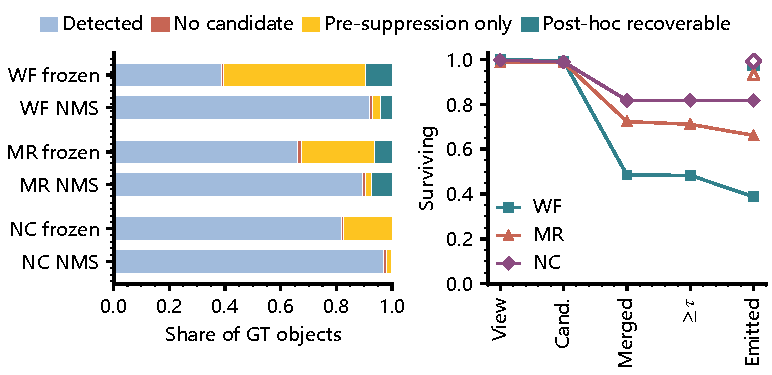
\includegraphics[width=0.98\textwidth,height=0.8\textheight,keepaspectratio]{../figures/fig_yst.pdf}
    \caption{Native-resolution source re-check on Yellow Sticky Traps (85 held-out test images; WF 1882, MR 584, NC 257 objects). Left: outcome partition per class under the frozen pipeline and under an NMS read-out with a 300-box cap. Right: stage survival per class under the frozen pipeline; hollow markers: oracle full-view read-out.}
    \label{fig:yst}
\end{figure}




